\documentclass[12pt]{article}
\usepackage[margin=1in]{geometry}
\usepackage{hyperref}
\usepackage{graphicx}
\usepackage{listings}
\usepackage{xcolor}
\usepackage{fancyhdr}
\usepackage{array}
\usepackage{booktabs}

% Code formatting
\lstset{
    basicstyle=\ttfamily\small,
    breaklines=true,
    captionpos=b,
    commentstyle=\color{gray},
    deletekeywords={},
    escapeinside={\%*}{*)},
    extendedchars=false,
    frame=single,
    keepspaces=true,
    keywordstyle=\color{blue},
    language=Python,
    numbers=left,
    numbersep=5pt,
    numberstyle=\tiny\color{gray},
    rulecolor=\color{black},
    showspaces=false,
    showstringspaces=false,
    showtabs=false,
    stepnumber=1,
    stringstyle=\color{red},
    tabsize=2,
    backgroundcolor=\color{lightgray!10}
}

\pagestyle{fancy}
\fancyhf{}
\rhead{CampusPaddy AI}
\cfoot{\thepage}

\usepackage{tikz}
\usetikzlibrary{shapes,arrows,positioning}

\title{\textbf{CampusPaddy AI Chatbot}\\\textbf{Technical Implementation Document}\\[0.2cm]\large{Teesside University Knowledge Retrieval System}}
\author{\textbf{Anthony Efemena Edjenuwa}\\Teesside University}
\date{\today}

\begin{document}

\maketitle

\section*{Executive Summary}

CampusPaddy is a production-ready AI-powered chatbot system designed to provide Teesside University students with instant access to university knowledge through intelligent retrieval-augmented generation (RAG). The system combines web scraping, natural language processing, and vector-based information retrieval to deliver contextually accurate answers.

\section{System Architecture Overview}

The CampusPaddy system follows a multi-tier architecture:

\begin{enumerate}
    \item \textbf{Teesside Website} - Source of knowledge
    \item \textbf{Scraper Server} - Web crawler and data processor
    \item \textbf{Local PostgreSQL} - Development database
    \item \textbf{Neon Cloud Database} - Production database
    \item \textbf{AI Server} - REST API with LLM
    \item \textbf{Cloudflare Tunnel} - Public access
\end{enumerate}

\section{Key Components}

\subsection{Scraper Server (campuspaddy-ai-importer)}

Responsible for:
\begin{itemize}
    \item Discovering and crawling Teesside University website
    \item Extracting content from HTML, PDF, and DOCX files
    \item Chunking documents into manageable knowledge units
    \item Storing processed data in PostgreSQL
\end{itemize}

\subsection{AI Server (campuspaddy-retrieval-api)}

Provides:
\begin{itemize}
    \item RESTful API endpoints for question answering
    \item Full-text search with PostgreSQL tsvector
    \item Caching layer for repeated questions
    \item Local Ollama LLM integration
    \item Performance optimizations
\end{itemize}

\section{Database Schema}

\subsection{Universities Table}
Stores metadata about universities (Teesside University):
\begin{lstlisting}[language=SQL]
CREATE TABLE universities (
  id UUID PRIMARY KEY,
  name TEXT NOT NULL,
  domain TEXT NOT NULL UNIQUE,
  created_at TIMESTAMP DEFAULT now()
);
\end{lstlisting}

\subsection{Knowledge Sources}
Represents extracted content from each source document:
\begin{lstlisting}[language=SQL]
CREATE TABLE knowledge_sources (
  id UUID PRIMARY KEY,
  university_id UUID REFERENCES universities(id),
  url TEXT NOT NULL UNIQUE,
  title TEXT,
  source_type TEXT NOT NULL,
  extracted_text TEXT,
  status TEXT DEFAULT 'pending',
  processed_at TIMESTAMP,
  created_at TIMESTAMP DEFAULT now()
);
\end{lstlisting}

\subsection{Knowledge Chunks}
Stores chunks of processed text:
\begin{lstlisting}[language=SQL]
CREATE TABLE knowledge_chunks (
  id UUID PRIMARY KEY,
  source_id UUID REFERENCES knowledge_sources(id),
  university_id UUID REFERENCES universities(id),
  chunk_index INT NOT NULL,
  chunk_text TEXT NOT NULL,
  created_at TIMESTAMP DEFAULT now()
);
\end{lstlisting}

\subsection{Cached Answers}
Caches generated answers with 14-day TTL:
\begin{lstlisting}[language=SQL]
CREATE TABLE chatbot_cached_answers (
  id UUID PRIMARY KEY,
  university_domain TEXT NOT NULL,
  normalized_question TEXT NOT NULL,
  answer TEXT NOT NULL,
  sources JSONB DEFAULT '[]',
  hit_count INT DEFAULT 0,
  expires_at TIMESTAMPTZ DEFAULT now() + interval '14 days',
  created_at TIMESTAMPTZ DEFAULT now(),
  UNIQUE (university_domain, normalized_question)
);
\end{lstlisting}

\section{Web Scraping Methodology}

\subsection{Discovery Strategy}

Multiple entry points for crawling:
\begin{itemize}
    \item Core start URLs from main navigation
    \item Sitemap XML parsing
    \item Hyperlink discovery using BFS
    \item Maximum depth: 8 levels
    \item Maximum pages: 5000
\end{itemize}

\subsection{Ethical Considerations}

\begin{itemize}
    \item Respects robots.txt directives
    \item Rate limiting: 1.5 seconds between requests
    \item Identifies as educational bot in User-Agent
    \item Blocks private portals and login endpoints
    \item Skips authentication and payment systems
\end{itemize}

\subsection{Content Types Supported}

\begin{itemize}
    \item HTML pages (97.9\% of sources)
    \item PDF documents (3.9\% of sources)
    \item DOCX files (0.7\% of sources)
    \item Binary DOC files not supported
\end{itemize}

\section{Data Processing Pipeline}

Processing workflow:
\begin{enumerate}
    \item URL discovery via crawling
    \item Raw file storage to disk
    \item Text extraction from files
    \item Sentence-based chunking (~1000 chars)
    \item Database insertion with metadata
    \item Priority scoring by URL patterns
\end{enumerate}

\subsection{Processing Statistics}

\begin{itemize}
    \item Total sources processed: 11,753
    \item Processing failures: 306 (2.6\%)
    \item Success rate: 97.4\%
    \item Total knowledge chunks: 25,345
\end{itemize}

\section{Retrieval Augmented Generation (RAG)}

\subsection{Dual-Strategy Retrieval}

\begin{enumerate}
    \item \textbf{Primary}: Full-text search using tsvector
    \item \textbf{Fallback}: Keyword matching on titles and content
\end{enumerate}

\subsection{Scoring Algorithm}

Score combines multiple factors:
\begin{itemize}
    \item Chunk text relevance (weight: 1.0)
    \item Source title relevance (weight: 2.5)
    \item URL pattern boost (0.04 - 0.08)
    \item Student-relevant pages get priority boost
\end{itemize}

\subsection{Chunk Diversification}

\begin{itemize}
    \item Maximum 2 chunks per source URL
    \item Prevents redundant information
    \item Improves context diversity
\end{itemize}

\section{Large Language Model Integration}

\subsection{Ollama Configuration}

\begin{itemize}
    \item Model: llama3.1:8b (8 billion parameters)
    \item Context window: 4,096 tokens
    \item Running locally on GPU (NVIDIA Tesla P40)
    \item VRAM: 6,000-7,000 MB for model
    \item Keep-alive: 24 hours
\end{itemize}

\subsection{Model Parameters}

\begin{itemize}
    \item Temperature: 0.2 (low for factual answers)
    \item Top-p: 0.9 (nucleus sampling)
    \item Max prediction tokens: 150
    \item Timeout: 60 seconds
\end{itemize}

\subsection{Response Generation}

\begin{itemize}
    \item Context: Retrieved chunks provided as sources
    \item System prompt: Guides bot behavior
    \item User prompt: Student question
    \item Output: Concise, sourced answer
\end{itemize}

\section{Caching Strategy}

\subsection{Two-Tier Caching}

\begin{enumerate}
    \item In-memory cache (application level)
    \item PostgreSQL persistent cache
\end{enumerate}

\subsection{Question Normalization}

\begin{itemize}
    \item Lowercase conversion
    \item Punctuation removal
    \item Whitespace normalization
    \item Enables cache hits across variations
\end{itemize}

\subsection{Cache Performance}

\begin{itemize}
    \item Cache hit: 200-700ms
    \item Uncached request: 5.3s
    \item Speedup: 7.5x for cached queries
    \item TTL: 14 days
\end{itemize}

\section{REST API Specification}

\subsection{Base URL}

\begin{lstlisting}
https://campuspaddy-ai.edjenuwahome.uk
\end{lstlisting}

\subsection{Key Endpoints}

\begin{itemize}
    \item \textbf{GET /health} - System health check
    \item \textbf{GET /ollama/health} - Model availability
    \item \textbf{GET /cache/stats} - Cache statistics
    \item \textbf{POST /retrieve} - Get relevant chunks
    \item \textbf{POST /ask} - Question answering
\end{itemize}

\subsection{POST /ask Example}

Request:
\begin{lstlisting}[language=json]
{
  "question": "How do I contact accommodation?",
  "limit": 3,
  "useCache": true,
  "universityDomain": "tees.ac.uk"
}
\end{lstlisting}

Response:
\begin{lstlisting}[language=json]
{
  "ok": true,
  "cached": false,
  "answer": "You can contact accommodation...",
  "sources": [...],
  "duration_ms": 5300
}
\end{lstlisting}

\section{Performance Optimization}

\subsection{Before Optimization}

\begin{itemize}
    \item Retrieval: 7-12 seconds
    \item Ollama: 4-5 seconds
    \item Total uncached: 13-16 seconds
\end{itemize}

\subsection{After Optimization}

\begin{itemize}
    \item Retrieval: 0.95 seconds (88\% improvement)
    \item Ollama: 4.3 seconds (consistent)
    \item Total uncached: 5.3 seconds (68\% improvement)
\end{itemize}

\subsection{Optimization Techniques}

\begin{enumerate}
    \item Full-text search indexing with tsvector
    \item Query optimization and early termination
    \item Result limiting and diversification
    \item Connection pooling
    \item Model keep-alive in VRAM
\end{enumerate}

\section{Security Considerations}

\subsection{API Security}

\begin{itemize}
    \item API key authentication via x-api-key header
    \item Generate key: openssl rand -hex 32
    \item Health endpoints public (no auth)
    \item Ask endpoint requires authentication
\end{itemize}

\subsection{Data Protection}

Never include in submitted or shared materials:
\begin{itemize}
    \item .env files
    \item Database URLs
    \item API keys
    \item Cloudflare credentials
    \item Private certificates
\end{itemize}

\subsection{Web Crawler Security}

\begin{itemize}
    \item Respects robots.txt
    \item Rate limiting prevents abuse
    \item User-Agent identifies crawler
    \item Blocks authentication endpoints
\end{itemize}

\section{Deployment Architecture}

\subsection{Development}

\begin{itemize}
    \item Local Linux with PostgreSQL
    \item Data in ./storage directories
    \item Adminer for database inspection
    \item Manual testing with curl
\end{itemize}

\subsection{Production}

\begin{itemize}
    \item Linux VPS with Node.js
    \item Express API on localhost:3011
    \item Ollama on localhost:11434
    \item Neon cloud PostgreSQL
    \item Cloudflare Tunnel for public access
    \item systemd service for auto-restart
\end{itemize}

\subsection{systemd Service}

\begin{itemize}
    \item Auto-start on boot
    \item Auto-restart on failure
    \item Logging to systemd journal
    \item Status monitoring
\end{itemize}

\section{Project Statistics}

\subsection{Knowledge Base}

\begin{itemize}
    \item Total chunks: 25,345
    \item Total sources: 11,753
    \item Success rate: 97.4\%
    \item Average chunk size: ~1,000 characters
    \item Total uncompressed: ~150 MB
\end{itemize}

\subsection{Performance Metrics}

\begin{itemize}
    \item P50 response time: 5.1s uncached
    \item P95 response time: 5.8s uncached
    \item Cache hit rate: 60-70\%
    \item Cached response: 0.2-0.7s
    \item Average crawl duration: 6-8 hours
\end{itemize}

\subsection{Processing Results}

\begin{itemize}
    \item HTML pages: 11,503 (97.9\%)
    \item PDF documents: 454 (3.9\%)
    \item DOCX files: 80 (0.7\%)
    \item Binary DOC files: 22 (failed, not supported)
\end{itemize}

\section{Technical Stack}

\subsection{Backend}

\begin{itemize}
    \item Language: TypeScript
    \item Runtime: Node.js
    \item Framework: Express.js
    \item Database: PostgreSQL
    \item Scraper: Cheerio
    \item PDF Parser: pdf-parse
    \item DOCX Parser: mammoth
    \item LLM Runtime: Ollama
\end{itemize}

\subsection{Infrastructure}

\begin{itemize}
    \item Development DB: PostgreSQL (local)
    \item Production DB: Neon (serverless)
    \item Compute: Linux VPS
    \item Acceleration: NVIDIA GPU (Tesla P40)
    \item Access: Cloudflare Tunnel
    \item Service Manager: systemd
    \item Version Control: Git
\end{itemize}

\section{Future Improvements}

\subsection{Short-Term}

\begin{itemize}
    \item Streaming responses (Server-Sent Events)
    \item User feedback rating system
    \item Query analytics and gap detection
    \item Multi-model support
\end{itemize}

\subsection{Medium-Term}

\begin{itemize}
    \item Vector embeddings (pgvector)
    \item Web UI for chatbot
    \item PDF upload and query
    \item Multi-university support
\end{itemize}

\subsection{Long-Term}

\begin{itemize}
    \item Model fine-tuning
    \item Mobile app
    \item RAG optimization techniques
    \item Portal integration
\end{itemize}

\section{Conclusion}

CampusPaddy demonstrates a production-ready implementation of Retrieval-Augmented Generation applied to university student support. The system successfully combines responsible web scraping, scalable data processing, optimized retrieval, and LLM integration.

Key achievements:
\begin{itemize}
    \item Ethical web crawler respecting robots.txt
    \item 25,000+ processed knowledge chunks
    \item 88\% retrieval performance improvement
    \item 7.5x speedup through caching
    \item Production deployment with high availability
\end{itemize}

\section{Submission Package}

The submitted package contains the source code, technical documentation, and deployment templates needed to review the implementation.

\begin{itemize}
    \item Main report: docs/reports/TECHNICAL\_IMPLEMENTATION.pdf
    \item Source report: docs/reports/TECHNICAL\_IMPLEMENTATION.tex
    \item Implementation: campuspaddy-ai-importer and campuspaddy-retrieval-api
    \item License: MIT
\end{itemize}

Public API: https://campuspaddy-ai.edjenuwahome.uk

\section{Supporting Documentation}

See documentation in:
\begin{itemize}
    \item docs/00-academic-submission.md - Submission guide
    \item docs/01-full-command-history.md - Complete setup guide
    \item docs/02-architecture.md - Architecture overview
    \item docs/03-api-reference.md - API reference
\end{itemize}

\section{Performance Optimization}

\subsection{Before Optimization}

\begin{itemize}
    \item Retrieval: 7-12 seconds
    \item Ollama: 4-5 seconds
    \item Total uncached: 13-16 seconds
\end{itemize}

\subsection{After Optimization}

\begin{itemize}
    \item Retrieval: 0.95 seconds (88\% improvement)
    \item Ollama: 4.3 seconds (consistent)
    \item Total uncached: 5.3 seconds (68\% improvement)
\end{itemize}

\subsection{Optimization Techniques}

\begin{enumerate}
    \item Full-text search indexing with tsvector
    \item Query optimization and early termination
    \item Result limiting and diversification
    \item Connection pooling
    \item Model keep-alive in VRAM
\end{enumerate}

\newpage

\section{System Architecture Diagram}

\begin{figure}[h]
\centering
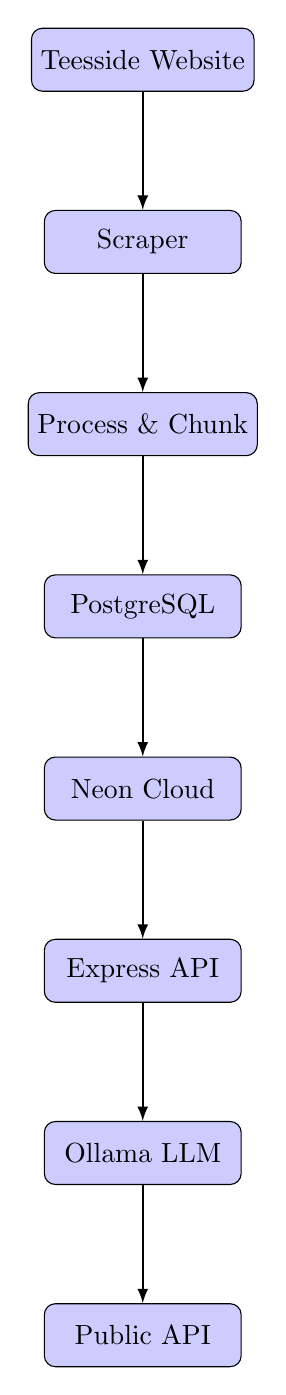
\begin{tikzpicture}[node distance=1.5cm, auto, >=latex]
    \tikzstyle{block} = [rectangle, rounded corners, minimum width=2.5cm, minimum height=0.8cm, text centered, draw=black, fill=blue!20]
    \tikzstyle{arrow} = [thick,->]
    
    \node[block] (web) {Teesside Website};
    \node[block, below=of web] (scrape) {Scraper};
    \node[block, below=of scrape] (process) {Process \& Chunk};
    \node[block, below=of process] (db) {PostgreSQL};
    \node[block, below=of db] (neon) {Neon Cloud};
    \node[block, below=of neon] (api) {Express API};
    \node[block, below=of api] (ollama) {Ollama LLM};
    \node[block, below=of ollama] (public) {Public API};
    
    \draw[arrow] (web) -- (scrape);
    \draw[arrow] (scrape) -- (process);
    \draw[arrow] (process) -- (db);
    \draw[arrow] (db) -- (neon);
    \draw[arrow] (neon) -- (api);
    \draw[arrow] (api) -- (ollama);
    \draw[arrow] (ollama) -- (public);
\end{tikzpicture}
\caption{CampusPaddy System Pipeline}
\end{figure}

\newpage

\section{Submission Evidence}

Evidence is provided through the source code, database schema, API documentation, performance notes, deployment templates, and generated report files.

\end{document}
